\documentclass[12pt]{article}
\usepackage{amsmath}
\usepackage{graphicx}
\usepackage{amsthm}
\usepackage{xepersian}
\settextfont[ExternalLocation]{XB Niloofar.ttf}
\begin{document}
\begin{center}
{\Huge ترکیب}\\
\vspace{3mm}
{\large صالح زارع زاده}
\end{center}
\section*{محتوا}
\begin{enumerate}
\item{تعداد ترکیبات  \lr{k} :
\begin{itemize}
\item[1.1]{نمونه ای از شمارش ترکیبات}
\item[1.2]{شمارش ترکیبات تایی\lr{k-}}
\end{itemize}
}
\item{تعداد ترکیبات با تکرار:
\begin{itemize}
\item[2.1]{مثال برای شمردن تعداد زیرمجموعه ها}
\end{itemize}
}
\item{منابع}
\end{enumerate}
\section{شمارش ترکیبات تایی\lr{k-}}
\rl{تعداد ترکیبات k از مجموعه S مشخص شده از عناصر غالباً در متون ترکیبی ابتدایی توسط \lr{C (n,k)} یا با یک تنوع مانند}$C_{k}^{n}$,$ {}_{n}C_{k}$,${}^{n}C_{k}$, $C_{{n,k}}$\rl{ یا حتی}$C_{n}^{k} $\rl{(فرم دوم در متون فرانسوی ، رومانیایی ، روسی ، چینی و لهستانی استاندارد بود (نیاز به استناد)). با این وجود ، در همان زمینه های ریاضی ، همان تعداد رخ می دهد ، جایی که به آن اشاره شده است }${\tbinom {n}{k}}$ \rl{(معمولا خوانده میشود انتخاب \lr{k از n})}\rl{; به ویژه در فرمول binom به عنوان ضریب اتفاق می افتد ، از این رو نام آن را ضریب دو جمله ای می گذارد. می توان تعریف کرد} ${\tbinom {n}{k}} $\rl{برای همه اعداد طبیعی k به یکباره توسط رابطه:}
$$(1+X)^n=\sum_{k\ge 0}{{\binom {n}{k}}X^k}$$
\rl{که از آن روشن است که}
$${\binom {n}{0}}={\binom {n}{n}}=1$$
\begin{figure}[h]
 \begin{center} \vspace{-5pt}
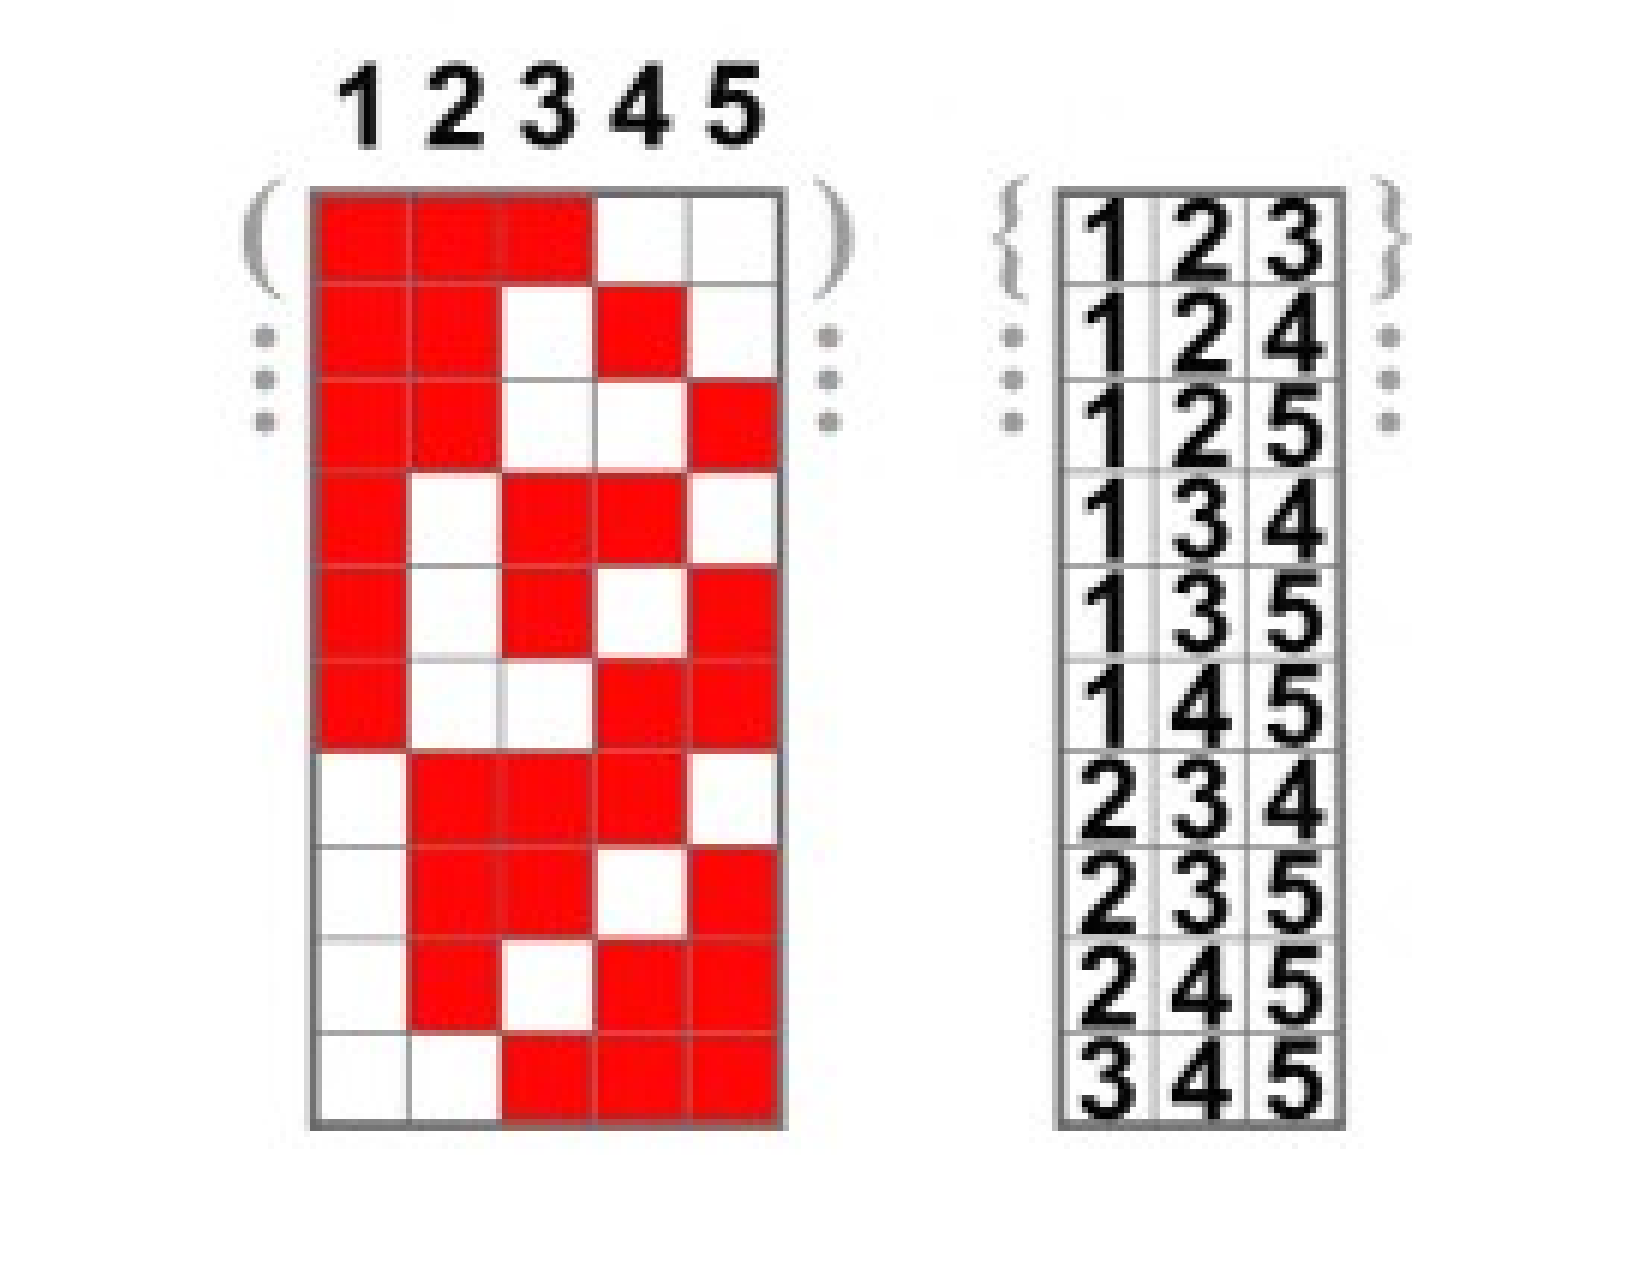
\includegraphics[scale=0.3]{1.pdf}
\caption{زیرمجموعه های ۳ عضوی از مجموعه ۵ تایی} \vspace{-10pt} 
\end{center}
\end{figure}
\rl{برای دیدن اینکه این ضرایب ترکیب K را از S در نظر می گیرند ، ابتدا می توانید مجموعه ای از متغیرهای مجزا $ X_s $ را برچسب گذاری شده توسط عناصر S S در نظر بگیرید و محصول را بر روی همه عناصر S گسترش دهید:}
$$\prod_{s\in S}{(1+X_s);}$$
\rl{این دارد}$ 2^n$\rl{اصطلاحات مجزا مربوط به تمام زیر مجموعه های S ، هر زیر مجموعه محصول از متغیرهای مربوطه را ارائه می دهد}$ X_s$\rl{. اکنون تنظیم همه}$ X_s$\rl{برابر با متغیر بدون علامت X ، به طوری که محصول می شود} $(1 + X)^n$\rl{، اصطلاح هر ترکیبی k از S می شود} $X^k$\rl{، به طوری که ضریب آن قدرت در نتیجه برابر با تعداد چنین ترکیبات K باشد.}\\
\rl{ضرایب دوتایی به صراحت از طرق مختلف قابل محاسبه است. برای به دست آوردن همه آنها برای موارد اضافی} $(1 + X)^n$\rl{، می توان از رابطه (بازگشت) علاوه بر موارد اساسی که قبلاً ارائه شده است استفاده کرد}
$${\binom {n}{k}}={\binom {n-1}{k-1}}+{\binom {n-1}{k}}$$
\rl{برای} $0 < k < n$\rl{، که از زیر دنبال می شود}$ (1 + X)^n = (1 + X)^{n-1}(1+X)$\rl{؛ این منجر به ساخت مثلث پاسکال می شود.
برای تعیین ضریب دوتایی فردی ، استفاده از فرمول عملی تر است}
$${\binom {n}{k}}=\frac{n(n-1)(n-2)\cdots (n-k)}{k!}$$
\rl{شمارنده تعداد k-permutations های n ، یعنی توالی های k عناصر مجزا S را نشان می دهد ، در حالی که مخرج تعداد این گونه k-permutations را می دهد که در صورت نادیده گرفتن ترتیب ، k- ترکیب مشابهی را ارائه می دهند.}\\
\rl{هنگامی که k از n / 2 تجاوز می کند ، فرمول فوق حاوی عواملی است که برای اعداد و مخرج مشترک هستند و لغو کردن آنها به این رابطه می دهد.}
$${\binom {n}{k}}={\binom {n}{n-k}}$$
\rl{برای}$0\le k\le n$\rl{این یک تقارن را بیان می کند که از فرمول دوجمله ای مشهود است ، و همچنین با گرفتن مکمل چنین ترکیبی ، می تواند از نظر ترکیبات k نیز قابل درک باشد.}$(n-k)$\rl{-ترکیب.}
\rl{سرانجام یک فرمول وجود دارد که این تقارن را مستقیماً به نمایش می گذارد و این ویژگی را دارد که به راحتی می توان به خاطر آورد:}
$${\binom {n}{k}}=\frac{n!}{(n-k)!k!}$$
\rl{که در آن! نشان دهنده فاکتوریل n. از فرمول قبلی با ضرب مخرج و شمارنده با (n - k) به دست می آید! بنابراین مطمئناً به عنوان روشی برای محاسبه آن فرمول فرومایه است.}\\\\
\rl{فرمول آخر را می توان بطور مستقیم و با در نظر گرفتن n! جایگشت همه عناصر S. هر یک از این تركیبات ها با انتخاب عناصر كیك اول خود ، به تركیب k می بخشند. انتخاب های تکراری زیادی وجود دارد: هر ترکیب ترکیبی از عناصر k اول در بین یکدیگر ، و عناصر نهایی (n - k) در بین یکدیگر ترکیب مشابهی را تولید می کنند. این تقسیم بندی را در فرمول توضیح می دهد.}\\\\
\rl{از فرمول بالا روابط بین اعداد مجاور در مثلث پاسکال را در هر سه جهت دنبال کنید:}
$${\binom {n}{k}}=
\begin{cases}
{\binom {n}{k-1}}\frac {n-k+1}{k} &\text{if } k>0\\
{\binom {n-1}{k}}\frac{n}{n-k}&\text{if }k<n\\
{\binom {n-1}{k-1}}\frac{n}{k}&\text{if } n,k>0
\end{cases}
$$
\rl{همراه با موارد اساسی}${\tbinom {n}{0}}=1={\tbinom {n}{n}}$\rl{، اینها امکان محاسبه پی در پی همه تعداد ترکیبات از همان مجموعه (یک ردیف در مثلث پاسکال) ، k-ترکیبی از مجموعه هایی با اندازه های در حال رشد و ترکیبات با یک مکمل از اندازه ثابت n - k را می دهد.}\\\\
{\large 1.1 نمونه ای از شمارش ترکیبات}\\\\
\rl{به عنوان یک مثال خاص ، می توان تعداد دست های پنج کارت را از یک عرشه استاندارد پنجاه و دو کارت محاسبه کرد:}
$${\binom {52}{5}}=\frac {52\times 51 \times 50 \times 49 \times 48}{5 \times 4 \times 3 \times 2 \times 1}=2,598,960$$\\\\
{\large 1.2 شمارش ترکیبات تایی\lr{k-}}\\\\
\rl{می توان همه ترکیبات k مجموعه ای از S عناصر n را به ترتیب ثابت شمارش کرد ، که باعث ایجاد حیات از فاصله زمانی از}${\tbinom{n}{k}}$\rl{ عدد صحیح با مجموعه ای از آن ترکیب K. با فرض اینکه S خود سفارش داده شده است ، به عنوان مثال} $ S = \{1 ، 2 ، \cdots ، n \} $ 
\begin{persian}، دو امکان طبیعی برای سفارش ترکیب k وجود دارد: با مقایسه اولین عناصر کوچک آنها (مانند تصاویر بالا) یا با مقایسه بزرگترین عناصر آنها ابتدا. گزینه دوم این مزیت را دارد که اضافه کردن یک عنصر بزرگتر جدید به S باعث تغییر قسمت اولیه شمارش نمی شود بلکه فقط ترکیب های جدید K را از مجموعه بزرگتر بعد از موارد قبلی اضافه کنید. با تکرار این روند ، شمارش می تواند به طور نامحدود با ترکیب K از مجموعه های همیشه بزرگتر گسترش یابد. اگر علاوه بر این ، فواصل اعداد صحیح برای شروع از 0 گرفته شود ، می توان ترکیب k را در یک مکان معین i در شمارش به راحتی از i محاسبه کرد ، و حیات بدست آمده به عنوان سیستم عدد ترکیبی شناخته می شود. همچنین در ریاضیات محاسباتی به عنوان "rank" / "rank" و "unranking" شناخته می شود.
\end{persian}
\lr{\\\\}
\rl{روشهای زیادی برای شمارش ترکیبات k وجود دارد. یک راه این است که از همه شماره های باینری کمتر از بازدید بازدید کنید} $2^n$\rl{آن دسته از اعداد را که دارای بیت k غیر صفر  است انتخاب کنید ، اگرچه این حتی برای n مثلا (بسیار کوچک) بسیار ناکارآمد است.}$ n = 20$\rl{ نیاز به بازدید حدود یک میلیون عدد دارد در حالی که حداکثر تعداد مجاز ترکیب k در حدود 186 هزار برای k = 10 است). موقعیت های این 1 بیت در چنین عددی ، k-ترکیبی خاص از مجموعه است}$\{ 1, …, n \}$\rl{. روش ساده و سریعتر ، ردیابی تعداد شاخص های k عناصر انتخاب شده ، با شروع است}$\{ 0,\cdots, k-1\}$\rl{(مبتنی بر صفر) یا }
$\{1,\cdots ,k\}$
\rl{(تک پایه ای) به عنوان اولین ترکیب ترکیبی مجاز و سپس بارها و بارها با افزایش آخرین عدد شاخص در صورتی که پایین تر از باشد ، به ترکیب k- مجاز بعدی منتقل می شود.} $n-1$\rl{(مبتنی بر صفر) یا n (یک پایه) یا آخرین عدد شاخص x که کمتر از عدد شاخص زیر است منهای یک است درصورتی که چنین شاخصی وجود داشته باشد و مجدداً تعداد شاخص ها را بعد از x به تنظیم مجدد کنید.}$\{x+1, x+2, …\}$\rl{.}\\\\\\\\\\\\\\\\\\\\\\
\section{تعداد ترکیبات با تکرار}
{\large  2.1 مثال برای شمردن تعداد زیرمجموعه ها}

\begin{table}[h]
\centering
\begin{tabular}{|c|c|c|c|}
\hline
شماره سطر. &مجموعه ۳ تایی & جواب & میله ها و ستاره ها \\
\hline
1&{1,1,1} &[3,0,0,0]&$\star \star \star |||$\\
\hline
2 &{1,1,2} &[2,1,0,0] &$\star \star |\star ||$\\
\hline
3&	{1,1,3}&	[2,0,1,0]&	$\star \star ||\star |$\\
\hline
4&	{1,1,4}&	[2,0,0,1]&	$\star \star |||\star$ \\
\hline
5&	{1,2,2}&	[1,2,0,0]&	$\star |\star \star ||$\\
\hline
6&	{1,2,3}&	[1,1,1,0]&	$\star |\star |\star |$\\
\hline
7&	{1,2,4}&	[1,1,0,1]&	$\star |\star ||\star$ \\
\hline
8&	{1,3,3}&	[1,0,2,0]&	$\star ||\star \star |$\\
\hline
9&	{1,3,4}&	[1,0,1,1]& $\star ||\star |\star$ \\
\hline
10&	{1,4,4}&	[1,0,0,2]&	$\star |||\star \star$ \\
\hline
11&	{2,2,2}&	[0,3,0,0]&	$|\star \star \star ||$\\
\hline
12&	{2,2,3}&	[0,2,1,0]&	$|\star \star |\star |$\\
\hline
13&	{2,2,4}&	[0,2,0,1]&	$|\star \star ||\star$ \\
\hline
14&	{2,3,3}&	[0,1,2,0]&	$|\star |\star \star |$\\
\hline
15&	{2,3,4}&	[0,1,1,1]&	$|\star |\star |\star$ \\
\hline
16&	{2,4,4}&	[0,1,0,2]&	$|\star ||\star \star$ \\
\hline
17&	{3,3,3}&	[0,0,3,0]&	$||\star \star \star |$\\
\hline
18&	{3,3,4}&	[0,0,2,1]&	$||\star \star |\star$ \\
\hline
19&	{3,4,4} &	[0,0,1,2]&	$||\star |\star \star$ \\
\hline 
20 &	{4,4,4} &	[0,0,0,3] &$|||\star \star \star$ \\
\hline
\end{tabular}
\end{table}
\lr{\\\\\\\\\\\\}
\begin{thebibliography}{10}
\begin{latin}
\bibitem{}
Benjamin, Arthur T.; Quinn, Jennifer J. (2003), Proofs that Really Count: The Art of Combinatorial Proof, The Dolciani Mathematical Expositions 27, The Mathematical Association of America, ISBN 978-0-88385-333-7
\bibitem{}
Brualdi, Richard A. (2010), Introductory Combinatorics (5th ed.), Pearson Prentice Hall, ISBN 978-0-13-602040-0
\bibitem{}
Erwin Kreyszig, Advanced Engineering Mathematics, John Wiley\& Sons, INC, 1999.
\bibitem{}
Mazur, David R. (2010), Combinatorics: A Guided Tour, Mathematical Association of America, ISBN 978-0-88385-762-5
\bibitem{}
Ryser, Herbert John (1963), Combinatorial Mathematics, The Carus Mathematical Monographs 14, Mathematical Association of America
\bibitem{}
https://en.wikipedia.org/wiki/Combination$\sharp$Number\_of\_k-combinations
\end{latin}
\end{thebibliography}




\end{document}